\documentclass[conference]{IEEEtran}
\usepackage{amsmath}
\usepackage{caption}
\usepackage{subcaption}
\usepackage{graphicx}
\usepackage{tikz}
\usepackage{algorithm}
\usepackage{algpseudocode}
\usepackage[font={small}]{caption}
\usepackage[final]{pdfpages}
\usepackage{multirow}
\usepackage{hyperref}


%\usepackage[table,xcdraw]{xcolor}


\renewcommand{\algorithmicrequire}{\textbf{Input:}}
\renewcommand{\algorithmicensure}{\textbf{Output:}}
%\algrenewcommand\alglinenumber[1]{\tiny #1:}
%\algsetup{linenosize=\small}

\usetikzlibrary{shapes.geometric, arrows}
\tikzstyle{startstop} = [rectangle, rounded corners, minimum width=3cm, minimum height=0.5cm,text centered, draw=black, fill=white]
\tikzstyle{process} = [rectangle, minimum width=3cm, minimum height=1cm,text width=3cm, text centered, draw=black, fill=white]
\tikzstyle{decision} = [circle, minimum size=1cm, text centered, text width=2cm, draw=black, fill=white]
\tikzstyle{io} = [trapezium, trapezium left angle=70, trapezium right angle=110, minimum width=3cm, minimum height=1cm, text centered,text width=3cm, draw=black, fill=white]
\tikzstyle{arrow} = [thick,->,>=stealth]

%\usepackage{mathtools}
\usepackage{float}
%\floatstyle{boxed}
%\restylefloat{figure}

\ifCLASSINFOpdf

\else
\fi
\hyphenation{op-tical net-works semi-conduc-tor}


\begin{document}
\title{Generation of Search-able PDF of the Chemical Equations segmented from Document Images}


%\author{\IEEEauthorblockN{Prerana Jana\IEEEauthorrefmark{1}, Anubhab Majumdar\IEEEauthorrefmark{1}, Sekhar K. Mandal\IEEEauthorrefmark{1}, Bhabatosh Chanda\IEEEauthorrefmark{2}}
%\IEEEauthorblockA{\IEEEauthorrefmark{1}
%Department of Computer Science and Technology\\
%Indian Institute of Engineering Science and Technology Shibpur, 
%India\\
%Email: \{prerana.jana, anubhabmajumdar93\}@gmail.com, sekhar@cs.becs.ac.in}
%\IEEEauthorblockA{\IEEEauthorrefmark{2}
%Electronics and Communication Sciences Unit \\
%Indian Statistical Institute,Kolkata,  India\\
%E-mail : chanda:at:isical.ac.in}
%}

\author{
\IEEEauthorblockN{Prerana Jana, Anubhab Majumdar, Sekhar Mandal}
\IEEEauthorblockA{Department of Computer Science and Technology\\
Indian Institute of Engineering Science and Technology 
\\Shibpur, India\\
Email: (prerana.jana, anubhabmajumdar93)@gmail.com\\sekhar@cs.iiests.ac.in}
\and
\IEEEauthorblockN{Bhabatosh Chanda}
\IEEEauthorblockA{Electronics and Communication Sciences Unit \\
Indian Statistical Institute
\\Kolkata,  India\\
E-mail : chanda@isical.ac.in}
}

%%%%%%%%%%%%%%%%%%%%%%%%%%%%%%%%%%%%%%%%

% make the title area
\maketitle

%%%%%%%%%%%%%%%%%%%%%%%%%%%%%%%%%%%%%%%%

\begin{abstract}
%\boldmath
 PDF format of scanned document images is not searchable. OCR tries to remedy this adversity by converting images or PDF files into
editable and searchable data, but it has it’s own limitations in presence of equations - both mathematical and chemical. OCR system for mathematical document images is already a major research area and has provided successful result. However,
chemical equation segmentation has been a less ventured road. In this paper we present a novel method for automated generation of searchable PDF format of segmented chemical equations from scanned document images by performing chemical symbol recognition and auto-correction of chemical compounds. We use existing OCR systems, pattern recognition, contextual data
analysis and a standard \LaTeX\ package to generate the chemical equation in searchable PDF format. The effectiveness of the
proposed method is demonstrated by testing it on 234 document images. 

\keywords Chemical equations, mathematical symbols, morphological operation. 
\end{abstract}

%%%%%%%%%%%%%%%%%%%%%%%%%%%%%%%%%%%%%%%%

\section{Introduction}
Text-based keywords are used for retrieving  documents from  WWW using search 
engines like Google.
%We use search engines like Google to find location of documents in WWW. Usually, text-based keywords are used for retrieving of documents.
 A large number of documents are being digitized today for the purpose of archival analysis, transmission and browsing. The existing OCR systems show high accuracy in interpreting text portions, but fail to properly process other components like graphics, half-tones, chemical and mathematical equations.

A few studies~\cite{blostein_97},~\cite{chan_00},~\cite{Garain_07} are directed toward math-symbol or math equation recognition
assuming that the math-zones are already marked. We, on the other hand, contend that a better approach is to segment the chemical equations from the mixed material thereby helping the future OCR activity to focus it’s processing only on specific
content. 

There are some methods that are used to reconstruct chemical molecules form scanned imge. They have used chemical datasets. Algorri et al.~\cite{algorri_07, algorri_07a} proposed a system that reconstruct chemical molecules from scanned document. They have used connected component analysis and their own vectorisation algorithm for character recognition. Connected components that are not recognised by the OCR engine, are used to produce a graph of vectors. A rule based approach reconstructs the molecule description from the vector graph and the character information. 
ChemReader~\cite{park_09} starts with connected component. Alphanumerics are  recognised using using the GOCR open source OCR tool. Graphical components are  identified using Hough transforms, corner detection and other bespoke algorithms.

In this paper we propose fully automated segmentation and detection technique of chemical equations present in
heterogeneous document images followed by generation of \LaTeX\ file of the segmented equations.

%%%%%%%%%%%%%%%%%%%%%%%%%%%%%%%%%%%%%%%%

\section{Proposed Work} 
\label{proposed_algo}
The proposed
method consists of four distinct steps and they are as follows: (i) Segmentation of displayed equations; (ii) Identification of
chemical equations; (iii) Auto correction of chemical compounds and the equation; and (iv) Generation of chemical equation in search-able PDF format.
 
\subsection{Segmentation of
displayed equations} A skew free heterogeneous binary image is the input of the proposed algorithm. The tables and graphics are
extracted out from the heterogeneous documents using the methods described in \cite{sekhar_06} and ~\cite{spc_07}. The rest of
the document contains normal text lines and displayed equations if any. Our main motivation is to classify chemical and non-chemical equations, we restrict our study to displayed equations only.

Major steps of segmentation of displayed equations (DE) are -  (i) Text line segmentation; (ii) Blob formation using morphological tools; and (iii) DE zone extraction.


%\begin{itemize}
%\item Text line segmentation
%\item Blob formation using morphological tools 
%\item DE zone
%extraction 
%\end{itemize} 
The details of the above steps are given in the following subsections.

\subsubsection{Text line segmentation} 
As the document image is skew free, the horizontal projection profile of the document page is taken to segment the
text line. %A part of a document page and its horizontal projection profile are shown in Fig.~\ref{H_PROJ}.
%\begin{figure}[h]
%\center\footnotesize 
%\begin{tabular}{c}
% 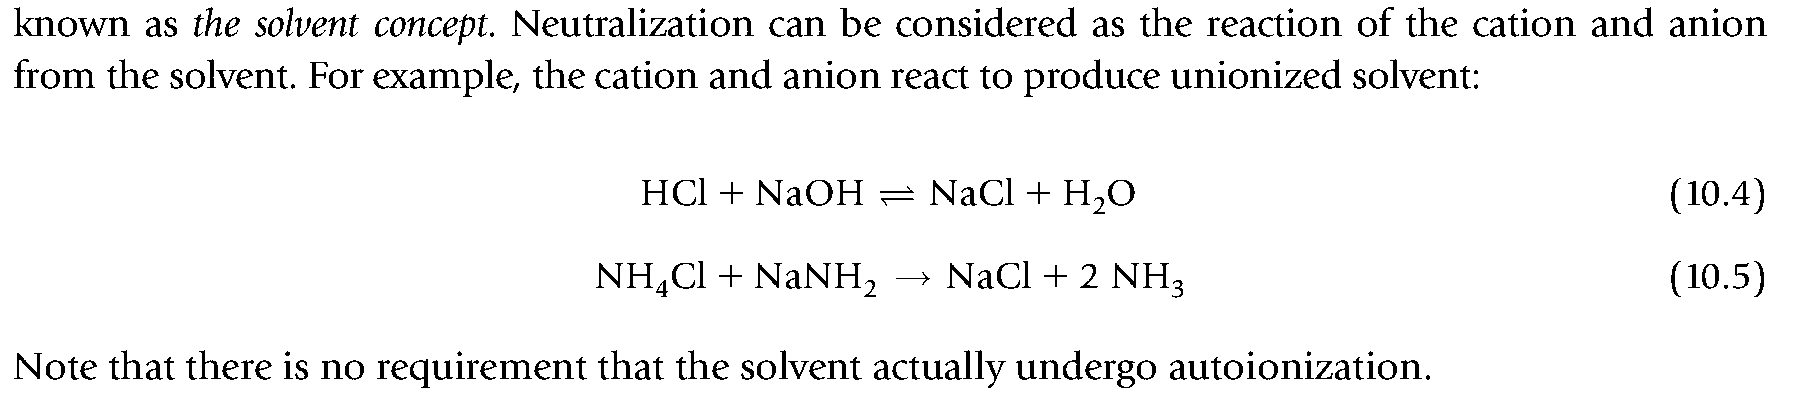
\includegraphics[width=0.35\textwidth]{simage.png} \\ (a) Image\\ 
% \includegraphics[width=0.35\textwidth]{hproj.png} \\ (b) Horizontal projection \\ 
%\end{tabular}
%\caption{ A document page and its horizontal projection profile.}
%\label{H_PROJ} 
%\end{figure} 

\subsubsection{Creation of word blobs} 

%\begin{figure}[h]
%\center\footnotesize
%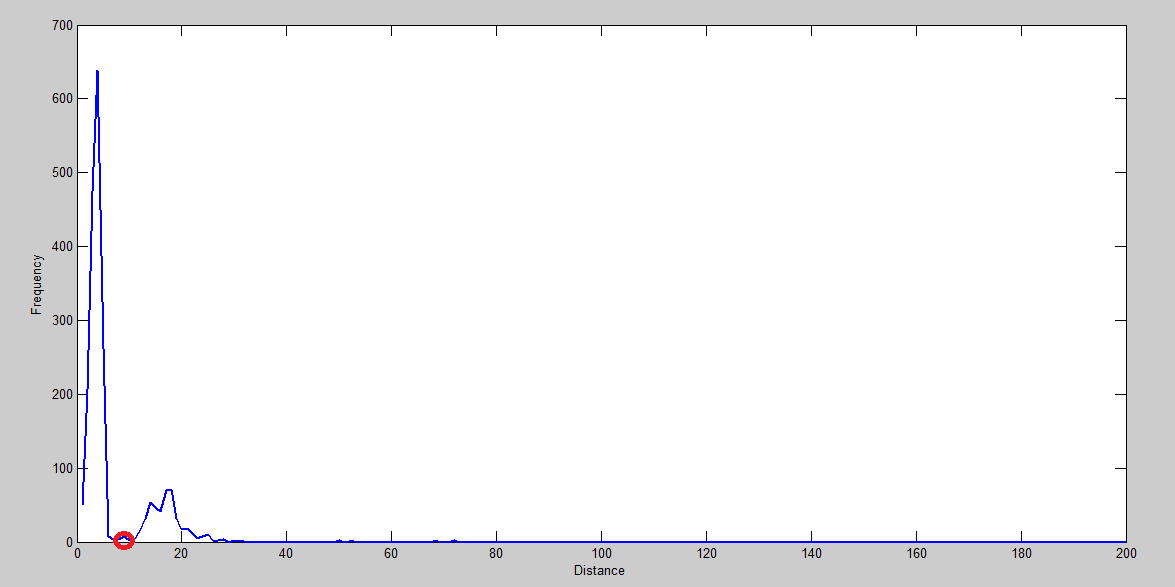
\includegraphics[width=0.3\textwidth]{histogram.png}
%\caption{Distance histogram of the image shown in Fig.~\ref{H_PROJ} (a) } 
%\label{hist} 
%\end{figure}

\begin{figure}[h]
\center\footnotesize 
\begin{tabular}{|c|c|}
\hline
 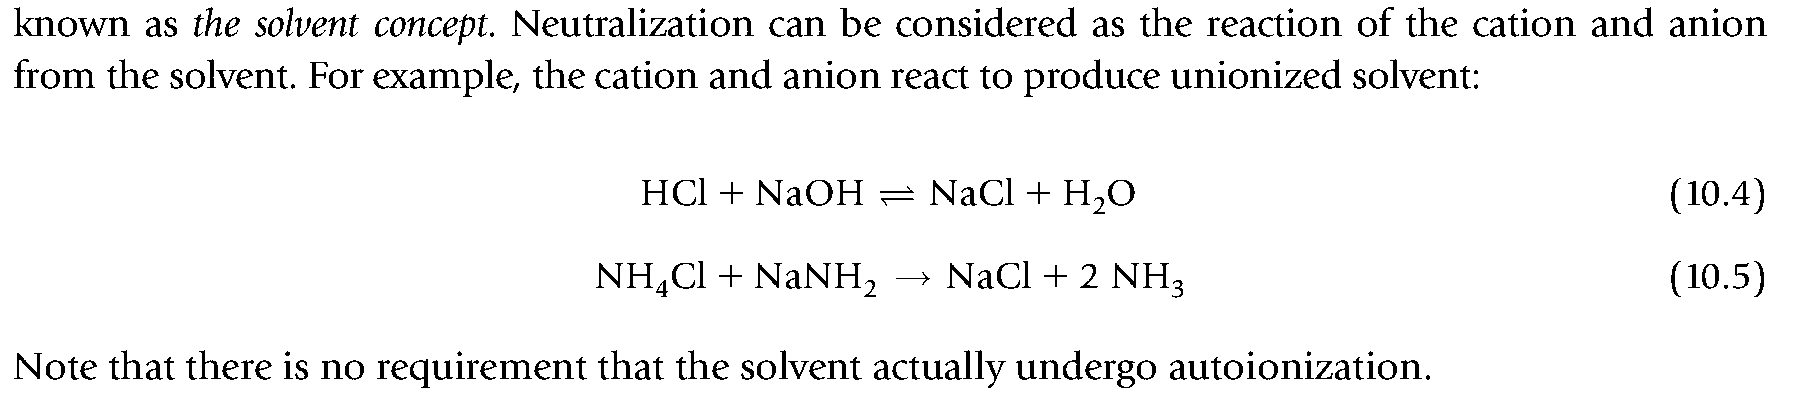
\includegraphics[width=0.2\textwidth]{simage.png} &
%\hline
 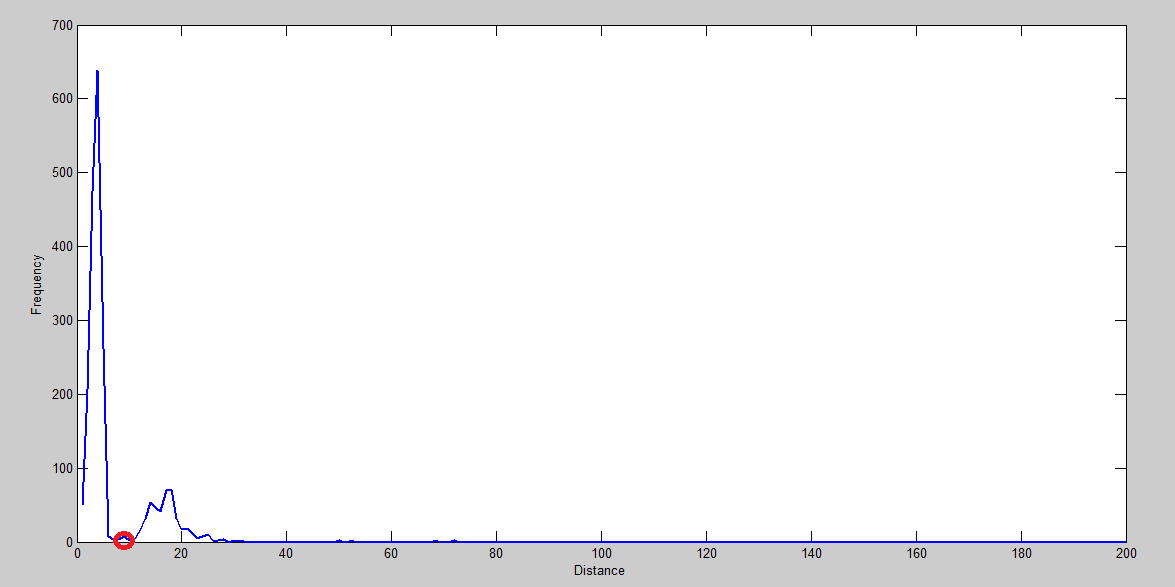
\includegraphics[width=0.2\textwidth]{histogram.png} \\
 (a) Image & (b) Distance Histogram\\
 \hline
\end{tabular}
\caption{ A document page and its distance histogram.}
\label{hist} 
\end{figure} 
%\begin{figure}[h]\center\footnotesize
%\begin{tabular}{c  c }
%%\hline 
% 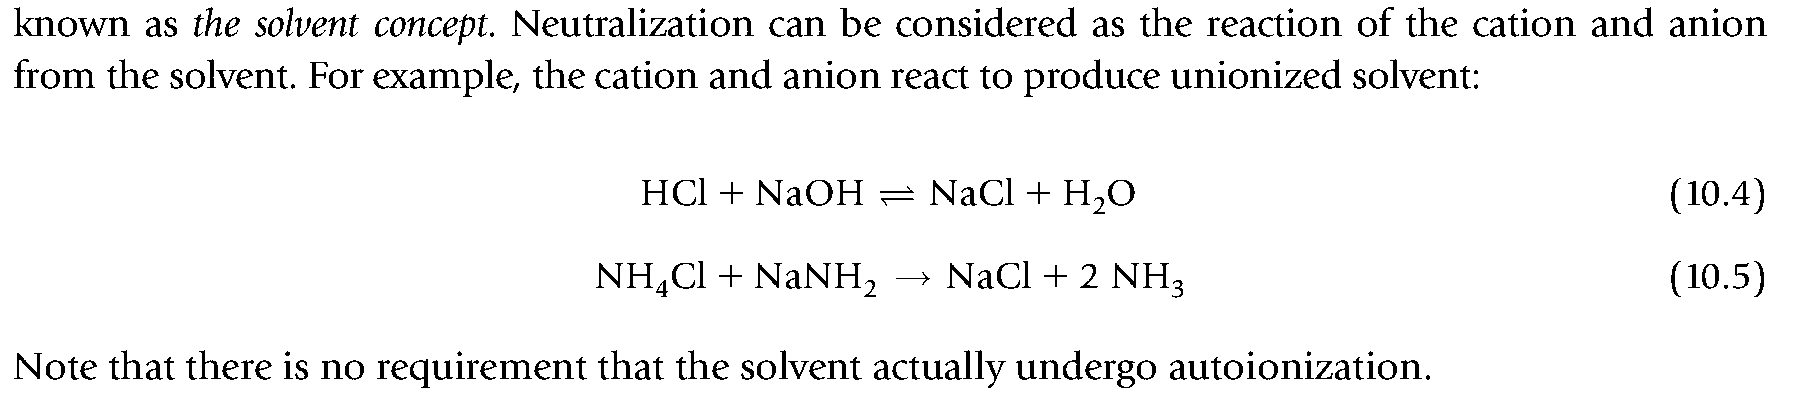
\includegraphics[width=0.3\linewidth]{simage.png}&  
% 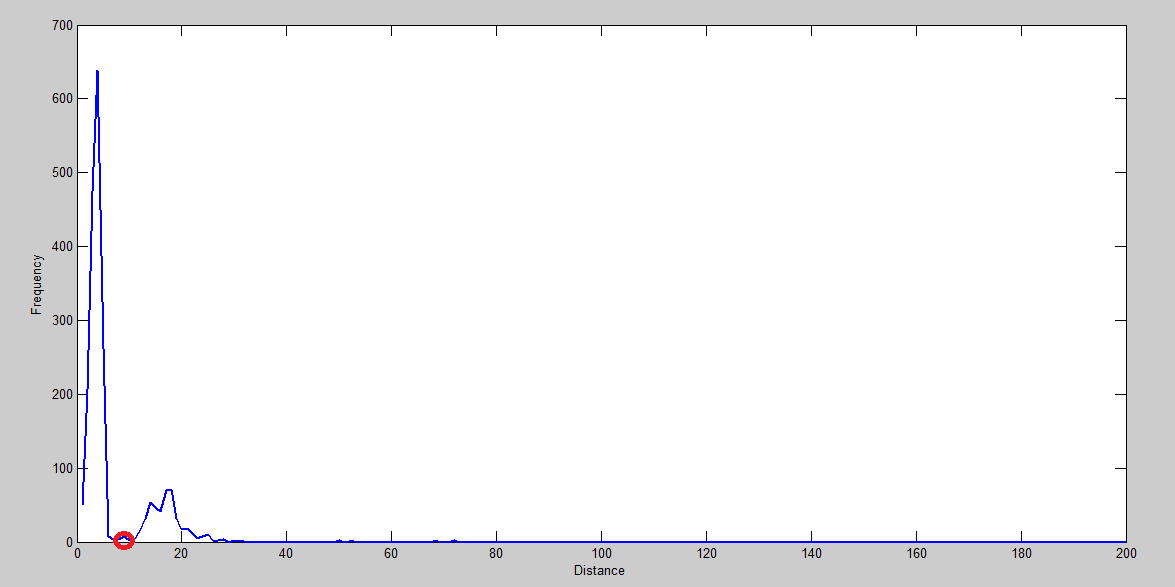
\includegraphics[width=0.3\linewidth]{histogram.png}& \\
%(a)&(b)\\
% \end{tabular} 
% \caption{(a). Arrow with reactants over it. (b). Bounding Box of the arrow. (c). After removal of smaller components}
% \label{fig:arrow_error}
%\end{figure}

This is done by coalescing the characters in a word using morphological closing operation. Such character coalescing process depends on the accuracy in detecting the normal character gap. The component analysis is done first. Let $C_a$ and $C_b$ be the two consecutive connected
components in a text line. $L_b$ is the left most x coordinate of $C_b$ and $R_a$ is the right most x coordinate of $C_a$. A distance function $D$ is defined as  $D = L_b - R_a$. The histogram of $D$ is obtained (see Fig.~\ref{hist}). The blob
formation requires information on inter-word gap. The distance histogram is a multi-modal histogram. The first peak is
corresponding to the character gaps. Our intention is to find out character gaps in running texts of a document page so that
we can combine the consecutive characters into a single blob. Hence, we consider the upper boundary ($l$) of the first hump as
the length of structuring element. Morphological close operation with a structuring element of size ($l\times 1$) will form the
blobs. The result of blob formation is shown in Fig.~\ref{BLOB_FORM}. 
\begin{figure}[h]
\center\footnotesize
\begin{tabular}{|c|} 
\hline
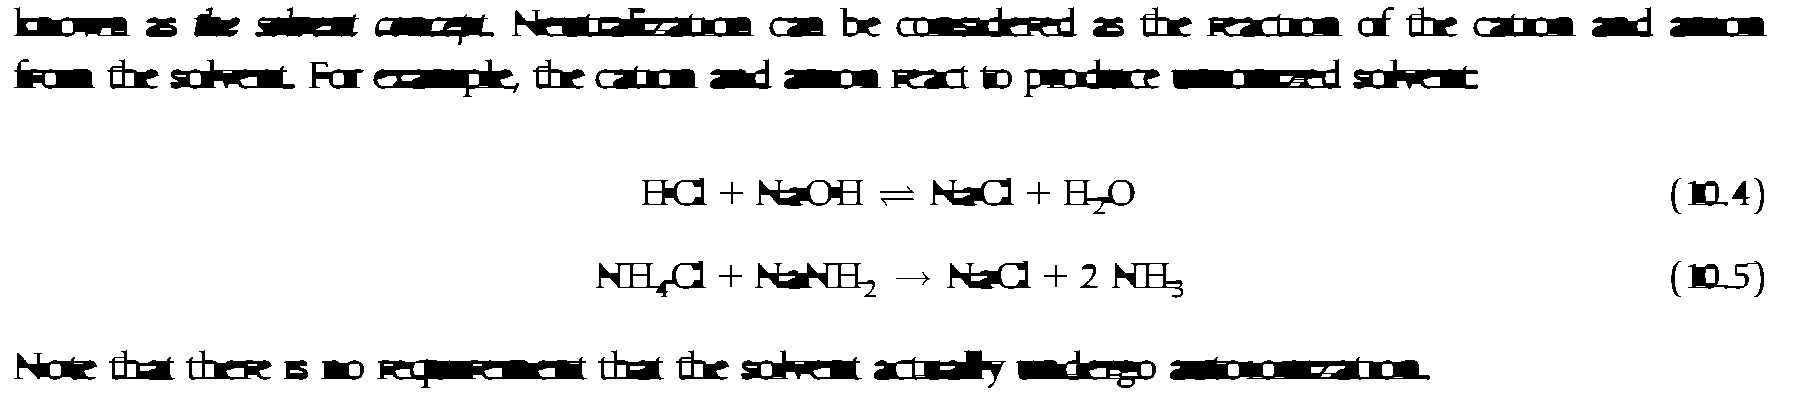
\includegraphics[width=0.3\textwidth]{blob.png}\\
\hline
\end{tabular}
\caption{Blob formation of the image shown in Fig.~\ref{hist}(a). } 
\label{BLOB_FORM} 
\end{figure}
\subsubsection{DE zone extraction} 
\label{DEZONE}
We have considered the set of operators that is commonly used both in chemical equations as well as mathematical equations to fulfil our aim to classify displayed zones containing chemical and non-chemical equations. After blob formation, small component like dots of \emph{i and j} are eliminated on the basis of area. The region, corresponding to each blob is considered from the original image and the
number of connected component(s) present in that region is counted. If the number of components is more than one that blob is not an operator and is removed from the  blob image.
% (see Fig.~\ref{single_com}). %Fig.~\ref{BLOB_FORM}.
%\begin{figure}[h]
%\center\footnotesize 
%\begin{tabular}{c}
%\includegraphics[width=0.3\textwidth]{singlechar.png} 
%\end{tabular} 
%\caption{Single components extracted from the blob image shown in Fig.~\ref{BLOB_FORM}} 
%\label{single_com}
%\end{figure} 
The remaining components in the blob image are operators along with some alphanumerics like $‘a’$, $‘A’$, $‘(’$, etc. The logical AND operation is performed between the blob image and the original image. The Euler number of the operators that we have considered is 1 (one) and based on this feature some of the alphanumerics are discarded. This image is denoted by $I_s$.
Width ($w$) and height ($h$) of each component in $I_s$ are determined. The components  are divided into two classes based on the ratio of $w, h$;
(i) {\em thin class} ($\frac{w}{h}$ $> 2$) and (ii) {\em regular class} ( $0.8 <$ $\frac{w}{h}$ $< 1.3$). 
Some instances of the \emph{thin}  and \emph{regular classes} are (-,  $\rightarrow$, $\leftarrow$, $\leftrightarrow$,  $\rightharpoonup$, $\leftharpoondown$, $\sim$, etc.) and  ( +, $\bullet$, X $\times$, etc) respectively. 

The number of \emph{on pixels}($N_p$) and number of \emph{off pixels} ($N_w$) within each bounding box of the thin components are calculated. 
Morphological opening operation is performed on {\em thin class} with a line like structuring element (SE) of length $\frac{w}{2}$.
If the output of the opening operation has a single component, then  thinning is performed on the corresponding original component.
Next, the number of end points of each thinned component is checked, if the number of end points is two  and $\frac{N_p}{N_w} > 0.8$, then the component under test is a `-' sign. If the number of end points is greater than two, then  element is an arrow. We need to identify the direction of the arrowhead for its correct representation in  \LaTeX\ file. The direction of arrowhead is identified by measuring the height of the arrow element near its two ends. 

From the \emph{regular class} our objective is to identify the `+' sign
and it is detected using the following rules: \\
(i)  Horizontal and Vertical Projection Profile of each component is considered;
(ii) Ratio of  $maxProj$, $D$ and ratio of $maxIndex$, $(M_l)$
%$\frac{maxProj}{D}$ and ratio of $\frac{maxIndex}{(M_l)}$
are obtained where maxProj is the maximum horizontal or vertical projection value, maxIndex is the index of maxProj closest to $M_l$ and D is width (height) for horizontal (vertical) profile. Here, $M_l$ is y (x) coordinate of the middle point for  horizontal (vertical) profile. 
If  $0.9 < \frac{maxProj}{D} \leq 1$,  $0.9 < \frac{maxIndex}{M_l} \leq 1.2$ and $\frac{N_w}{N_p} > 3$, then the component under test is a `+' sign.
Where $N_w$ and $N_p$ are number of \emph{on pixels} and \emph{off pixels} along the 
diagonal direction of the bounding box of the component. All the threshold values used  here are selected based on our empirical study on 234 images.

To detect `=' or `$\rightleftharpoons$' one extra step is
required. 
%The operators having $f_a$ $\leq$ 0.6 are considered
%thin symbols
%(-,$\leftharpoondown$,$\rightharpoonup$,$\rightarrow$,$\leftrightarrow$).
For each `-' and right-arrow  symbol, a rectangular mask is
placed below the symbol to check if there is `-' and left-arrow respectively within
the mask; if  present, they are considered to form either an `=' or
`$\rightleftharpoons$' sign. Let the length of the symbol
be $l$. The area of the mask is ($l \times l/2$). 

The horizontal line separating the numerator and the denominator
is identified as its length is greater than the median length of
the operators. Two windows are placed above and below the
separating line to merge all the components within the windows
with the separating line to form a single logical line.
Otherwise, they would be treated as three consecutive text lines
and we will not be able to associate the intermediate
math-symbols (‘+’, ‘-’, ‘=’) to a single expression. The area of
the window is (length of the separating line)$\times$ (twice the
median width of the text lines).

\begin{figure}[h]
\center\footnotesize 
\begin{tabular}{|c|}
\hline
 
\includegraphics[width=0.3\textwidth]{equation.png} \\ (a)\\  
 
\includegraphics[width=0.3\textwidth]{equationOperands.png} \\ (b)\\  

\includegraphics[width=0.3\textwidth]{equationNumber.png} \\ (c) \\ 

\includegraphics[width=0.3\textwidth]{hrlsaRemoval.png} \\ (d) \\ 
\hline 
\end{tabular}
\caption{The output of H-RLSA on portion of an image (a) a part of an image; (b) same part without operators; (c) result of H-RLSA operation; (d) after equation number removal.}
\label{h-rlsa} 
\end{figure} 
Initially, all the text lines consisting at least one operator
are considered candidate displayed equations (CDE). The
operators are eliminated from CDE. The upper boundary ($u_v$) of
the second hump of distance histogram (Fig.~\ref{hist}(b)) is obtained which
represents the word gaps in the text line. For each CDE zone Run
Length Smoothing Algorithm in horizontal direction (H-RLSA) is
carried out. If the distance between two neighbouring components
is less than $u_v$, it means they belong to a same word and are
merged by H-RLSA. H-RLSA has a similar effect as of dilation of
black areas in horizontal direction. The characters in a word
are dilated and coalesced to the other characters of the same
word. The output of H-RLSA is shown in Fig.~\ref{h-rlsa}.

Equation numbers are common in the displayed equation zones.
These numbers have to be removed because for each CDE we have
counted the number of operators and corresponding other
components in the output of H-RLSA. If the number of components
$\le$ 2$\times$ number of operators, then the CDE is considered
displayed equation; otherwise some embedded formulae/equations
may exist in the line. To eliminate the equation number from the
output of H-RLSA the operators are moved to the output of H-RLSA
and the component analysis is done. From both ends distance
($d$) (see Fig. \ref{h-rlsa}(c))
 between the first two consecutive
components is measured and if $d$ $> 5\times$ $u_v$, then the
first component from the end is considered the equation number
and is removed. (see Fig. \ref{h-rlsa}(d).

\subsection{Identification of chemical equations} Each segment
of a displayed equation is divided into three zones; namely
upper zone, middle zone and lower zone (see
Fig.~\ref{sub_super}). To identify the three zones of a DE zone,
uppermost and lowermost co-ordinates of each connected component
below the same DE zone are also obtained. The median of
uppermost coordinate, and median of lowermost co-ordinate of
such components in DE zone are computed. A horizontal line,
called the baseline, is drawn through the median of lowermost
coordinates of components and this baseline separates the middle
zone and lower zone of DE zone. Similarly, the median of
uppermost co-ordinate of the components in the DE zone generates
a horizontal line. This horizontal line, called top line,
separates the middle and upper zones of the DE zone.

\begin{figure}[h]
\center\ 
\begin{tabular}{|c|} 
\hline
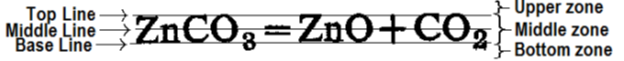
\includegraphics[width=0.3\textwidth]{supSub.png}\\
\hline
\end{tabular} 
\caption{Different zones of DE equation}
\label{sub_super} 
\end{figure} 
The subscripts in a DE zone
belong to lower-half of the middle zone and lower zone whereas
the superscripts belong to upper zone and upper-half of the
middle zone. Based on the location of the components in a DE
zone we have detected the subscripts and superscripts and are
separated from the DE zone. The operators are also separated
from DE zone.
 
Now, each displayed equation is an input to an OCR of MATLAB
R2014a. The OCR returns each DE zone as a text string. We made a
dictionary out of all the elements in the periodic table. An
important observation is that an element always starts with a
capital letter. Using this property, an element can be expressed
by a regular expression [A-Z][a-z]*. It means an element's
symbol starts with an upper case letter and may or may not have
one or more lower case letters. We have designed a parser to extract the
sub-string matching the regular expression mentioned above with
the following grammar: %\begin{center}
\small{
 $start \rightarrow capital.follow$\\ $follow \rightarrow small.follow | \in$\\
$capital \rightarrow A|B| \dots |X|Y|Z$\\  $small \rightarrow
a|b| \dots |x|y|z$\\ }
%\end{center} 
Each of the substring returned
by the parser is matched against the aforesaid dictionary and if
it is a positive match then that substring is considered as a
symbol of the chemical element. Let us consider, the number of
substrings extracted from the OCR output by the parser is {\em
n} and the number of positive matches the aforementioned
dictionary is {\em m}. If m:n ratio is more than a threshold
value $\beta$ then this DE is considered a Chemical Equation.
This threshold ($\beta$) is set to 0.7 by running our algorithm
on our dataset containing 1390 displayed equations. The reason
for the ratio not being 1 are (i) Limitations of OCR; (ii)
Touching and broken characters.
%%%%%%%%%%%%%%%%%%%%%%%%%%%%%%%%%%%%%%%%

The $\uparrow$ and $\downarrow$ are frequently used in chemical equation to represent the state of compounds and  are thus important to detect.
Let each chemical equation be denoted by $C_e$. Each $C_e$ zone is AND with $I_s$ which produces an output $I_o$. $I_o$ may contain  operators, single character elements and ($\uparrow$, $\downarrow$). The operators are removed from $I_o$ as they are already identified. For the rest of the components in $I_o$, we have checked whether the component is the starting character of the chemical equation, if not, then its immediate left neighbour in $C_e$ is checked. If the left neighbour is not an operator, then then component under test is  $\uparrow$ or $\downarrow$. The arrowhead direction is determined in the same way as right/left arrow in~\ref{DEZONE}.
\subsection{Auto correction of chemical compounds and the equation}

Next, auto correction is performed based on the chemical context as existing OCRs can not produce perfect result in case of chemical equations.  The output of H-RLSA  (see Fig.~\ref{h-rlsa} (d)) is taken as input here. 
Each character within a word blob is an input to the the OCR and the corresponding output  is stored in a cell and these cells form a string, S$_{chemical}$ for each word blob. For each superscript and subscript, `\^{}'  and  `\_' are inserted before them respectively in S$_{chemical}$.

 First, an error map is created based on the observation of OCR outputs of 280 chemical equations consisting of 1022 compounds (see Table \ref{table:errorTable}). Next, this table is stored into a hash map $H$ where the key is the OCR output and its value is the possible input set.
% Auto correction is performed based on this error hash map ($H$).
For example, if `$8$' is an erroneous OCR output for inputs `$g$', `$3$'and `$a$' (see Table \ref{table:errorTable}) then, in the hash map $H$, key is `$8$' and its corresponding value is [$g$, $3$, $a$] .

\begin{figure}[h]
\center\ 
\begin{tabular}{|c|} 
\hline
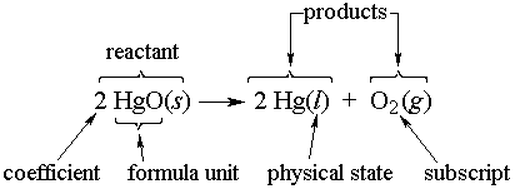
\includegraphics[width=0.25\textwidth]{chemEqParts.png}\\
\hline
\end{tabular} 
\caption{Different components of a chemical equation. }
\label{chemEqParts} 
\end{figure}  

 Each chemical compound in any equation (see Fig.~\ref{chemEqParts}) has the following format- [Coefficient]$^{[0,1]}$[Formula Unit][state]$^{[0,1]}$. Auto correction of the OCR output corresponding to each word blob includes the following steps - (i) Coefficient extraction; (ii) State separation; (iii)Auto correction of the formula unit; and (iv) Auto correction of the entire equation using Context Table.

%The details of the above steps are given in the following subsections (see Fig.~\ref{stateCorrection} and  ~\ref{autoCorrection} for an example).
\subsubsection{Coefficient Extraction}
Coefficient extraction is done by matching its regular expression $[2-9]^{+}[0-9]^{*}$ at the beginning of S$_{chemical}$ as it has numerical values. 
\subsubsection{State separation}
 There are 4 physical states of a chemical compound which are represented by `(s)', `(g)', `(l)' and `(aq)'. To detect the physical state of the compound,  regular expression [(][A-Za-z]$^{[1,2]}$[)] is used and the checking starts from the end of S$_{chemical}$. The matched substring ($S$) is extracted from  S$_{chemical}$ and Algorithm~\ref{alg:getAllCombs} is run. 
In this algorithm, $S$ and $H$  are taken as input and all possible $Combinations$ of corrected OCR output is produced by $GetAllCombinations$ (See Fig.~\ref{stateCorrection}). These $Combinations$ are compared with `s', `g', `l' and `aq'. If no match is found, the substring extracted from S$_{chemical}$ is a radical, not a state; else, we separate the state from the compound. 

\subsubsection{Auto correction of the formula unit}
After extracting coefficient and state, only the formula unit is left in S$_{chemical}$. 
The algorithm for autocorrection of each formula unit is done in two steps (See Algorithm~\ref{alg:getAllCombs} and~\ref{alg:findMatch}). First, Algorithm~\ref{alg:getAllCombs} is performed on the formula unit.
 Next, the output of Algorithm~\ref{alg:getAllCombs}($Combinations$) are matched against a nearly exhaustive list of all molecules, chemical compounds, radicals and atoms namely $ChemList$ collected from Wikipedia \footnote{\url{http://en.wikipedia.org/wiki/Dictionary_of_chemical_formulas}}.
%( reference: %http://en.wikipedia.org/wiki/List_of_compounds). 
%% check this part
If a perfect match is found, that match is considered as the $Corrected$ formula unit (See Fig.~\ref{autoCorrection}). But in case of no match, we go for
longest common substring(s) (LCS) match ($SubMatch$).% between $Combinations$ and $ChemList$ is computed and 
%the formula unit in $Chemlist$ having the longest common substring (LCS) with $Combinations$
 %is considered as $SubMatch$. 
If there is only one $SubMatch$ then the corresponding formula unit in $ChemList$ is considered as the $Corrected$  formula unit; else the $SubMatch$es are considered as $PossibleFormulaUnit$s. 
%All the $Corrected$ units are then included in the $FinalEquation$ (See Algorithm~\ref{alg:alg3}).
%See Fig.~\ref{autoCorrection} for an example.

\begin{table}
\captionof{table}{Part of the Error list}
\begin{center}
 \begin{tabular}{|| c | c ||}
 \hline
 correct input & all observed outputs given by OCR\\
 \hline
 g & 8 S\\
 \hline
O & 0\\
\hline
3 & 8 'E s w \\
\hline
a & 3. 21 8 El 8. \\
\hline
l & 1 I\\
\hline
s & S\\
 \hline
 \end{tabular}
 \end{center}
 \label{table:errorTable}
 \end{table}

\begin{figure}[h]
\center\ 
\begin{tabular}{|c|} 
\hline
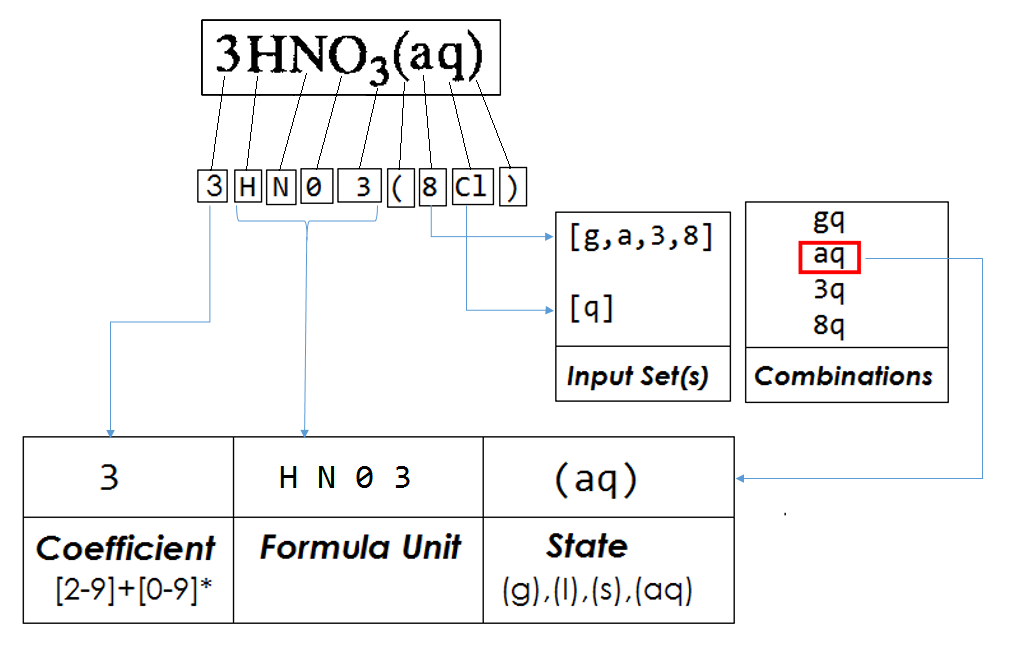
\includegraphics[width=0.23\textwidth]{stateCorrection.png}\\
\hline
\end{tabular} 
\caption{Extracting the formula unit, numeric coefficient and physical state from a chemical compound. }
\label{stateCorrection} 
\end{figure} 

\begin{figure}[h]
\center\ 
\begin{tabular}{|c|} 
\hline
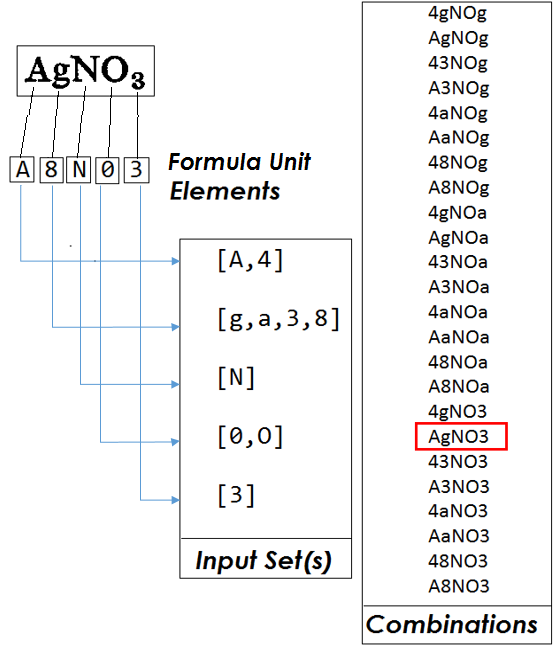
\includegraphics[width=0.23\textwidth]{autoCorrectionPictorial.png}\\
\hline
\end{tabular} 
\caption{Example of autocorrection of a formula unit. }
\label{autoCorrection} 
\end{figure} 

 

\begin{algorithm}
\small
\caption{Get All Combinations from the Error Hash Map}
\begin{algorithmic}[1]
	%\qinput{description of algorithm input}
\Procedure {GetAllCombinations}{$S$,$H$}
	%\State \textbf{Input:} {$CC, H$}
	%\State \textbf{Output:} {$Combinations$}
	\ForAll {$element(s) \in S$}
		\State $InputSet(s) \leftarrow H.Get(element)$ 
		\If {$InputSet(s)$ is $NULL$}
			\State $RETURN$ \Comment Not in Error Map
		\Else
			\If {$length(element) = 1 $}
				%\State $InputSet =\cup$  $element $
				\State $InputSets =\cup$ $[element]$ 
				\Statex \Comment Element might be correct output but still in the error list for other inputs
			\Else
				\State \textbf{Ignore}
				\Statex \Comment Input is one character, output length $>$ 1 means error
			\EndIf
		\EndIf
	\EndFor
\State $Combinations \leftarrow CartesianProduct(InputSets)$ %\Comment CartProd : Cartesian Product
\State  \textbf{Return} {$Combinations$}
\EndProcedure
\Statex
\end{algorithmic}
\label{alg:getAllCombs}
\end{algorithm}

\begin{algorithm}
\small
\caption{Find Match between ChemList and Combinations derived from Algorithm~\ref{alg:getAllCombs}}
\begin{algorithmic}[1]
\Procedure {FindMatch}{$ChemList$,$Combinations$} %\Comment $ChemList$ : nearly exhaustive list of all molecules and chemical compounds
	\ForAll{$Combinations$}
		\State \textbf{match} {with $ChemList$}
	\EndFor
	\If {\#(Match Found) = 1}
		\State $Corrected \leftarrow Match$
		\State  \textbf{Return} {$Corrected$}
	\ElsIf {\#(Match Found) = 0}
		\State $SubMatch \leftarrow \textbf{LCS}(Combinations,ChemList)$ 
		\Statex \Comment LCS : Longest Common Substring
		\If {{NumberOf}($SubMatch$)=1}
			\State $Corrected \leftarrow SubMatch$
			\State  \textbf{Return} {$Corrected$}
		\Else
			\State $PossibleFormulaUnit(s) \leftarrow SubMatch$
			\State  \textbf{Return} {$PossibleFormulaUnit(s)$}
		\EndIf
	\Else
		\State $PossibleFormulaUnits \leftarrow Matches$
		\State  \textbf{Return} {$PossibleFormulaUnit(s)$}
		\Statex \Comment Multiple matches
	\EndIf
\EndProcedure
\end{algorithmic}
\label{alg:findMatch}
\end{algorithm}

\subsubsection{Auto correction of the entire equation using Context Table}
Here, we have all the possible formula units and try to find out the $FinalEquation$ in the context of the equation itself. Algorithm~\ref{alg:alg3} takes all $Corrected$ and $PossibleFormulaUnit$s and returns the $FinalEquation$ by forming the Context Table. 
Chemical equations have the same periodic elements in the left hand side, called $Reactants$ as that in the right hand side, called $Products$. All the periodic elements follow the regular expression [A-Z][a-z]*. So, for each  $PossibleFormulaUnit$, the set of periodic elements in the $Reactants$, $P_{R}$ and in the $Products$, $P_{P}$ are computed and stored in the $Context Table$. When the set difference of $P_{R}$ and $P_{P}$ in the table is empty, that $PossibleFormulaUnit$ is considered as $Corrected$ and included in the $FinalEquation$ (See Fig.~\ref{context}). But if the above condition comes true for multiple possibilities, we cannot decide which of the possible formula units are actually in the original equation.The algorithm shows multiple $FinalEquation$s. This is considered an $ERROR$ case.
An example of formation of context table is demonstrated in  Fig.~\ref{context}. The co-effiecient and state (if any) are added with their correspodning $Corrected$ formula unit. The $FinalEquation$ is then converted to \LaTeX\  format using $mhchem$ package.

\begin{algorithm}
\small
\caption{Auto-Correction of the entire equation using chemical context table}
\begin{algorithmic}[1]
\Procedure {GetFinalEqn}{$PossibleFormulaUnit$,$Corrected$}
	\State {Include all $Corrected$ units in $FinalEquation$}
	\State{$Count  \leftarrow 0$}
	\For{every $PossibleFormulaUnit$}
		\State \textbf{compute}($P_{R}$)  
		\Statex \Comment{$P_{R}$ :  Set of periodic elements in Reactants}
		\State \textbf{compute}($P_{P}$)  \
		\Statex \Comment {$P_{P}$ : Set of periodic elements in Products}
		
		\If{$P_{R} - P_{P} = \emptyset $}
			\State $Corrected \leftarrow PossibleFormulaUnit$
			\State {Include that in the $FinalEquation$}
			\State $Count \leftarrow Count + 1$
		\EndIf
	\EndFor
	\If {$Count \geq 2 $}
		\State {Multiple $Corrected$ compounds}
		\State{Multiple $FinalEquations$}
		\Statex \Comment { $ERROR$}
	\EndIf
	\State  \textbf{Return} {$FinalEquation(s)$}
\EndProcedure
\end{algorithmic}
\label{alg:alg3}
\end{algorithm}

\begin{figure}[h]
\center\ 
\begin{tabular}{|c|} 
\hline
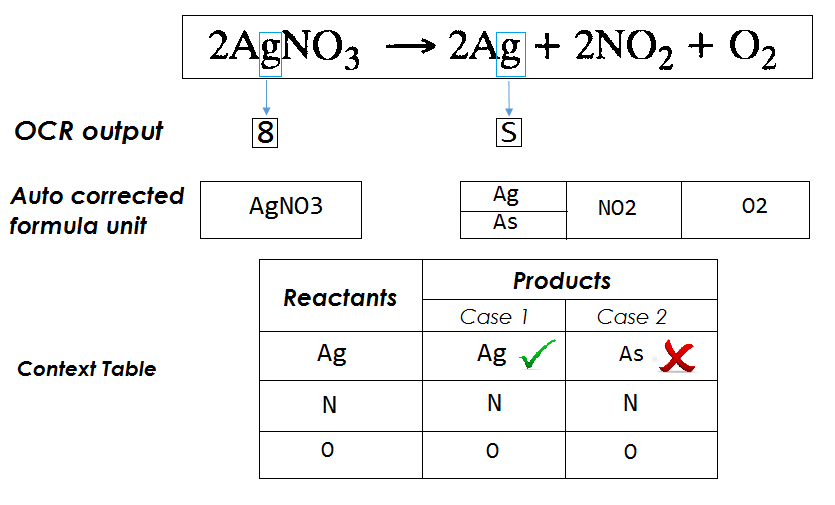
\includegraphics[width=0.25\textwidth]{equationContext.png}\\
\hline
\end{tabular} 
\caption{Formation of context table. }
\label{context} 
\end{figure}
\begin{figure}[]
\center\footnotesize
\begin{tabular}{ |c|c|}
\hline
 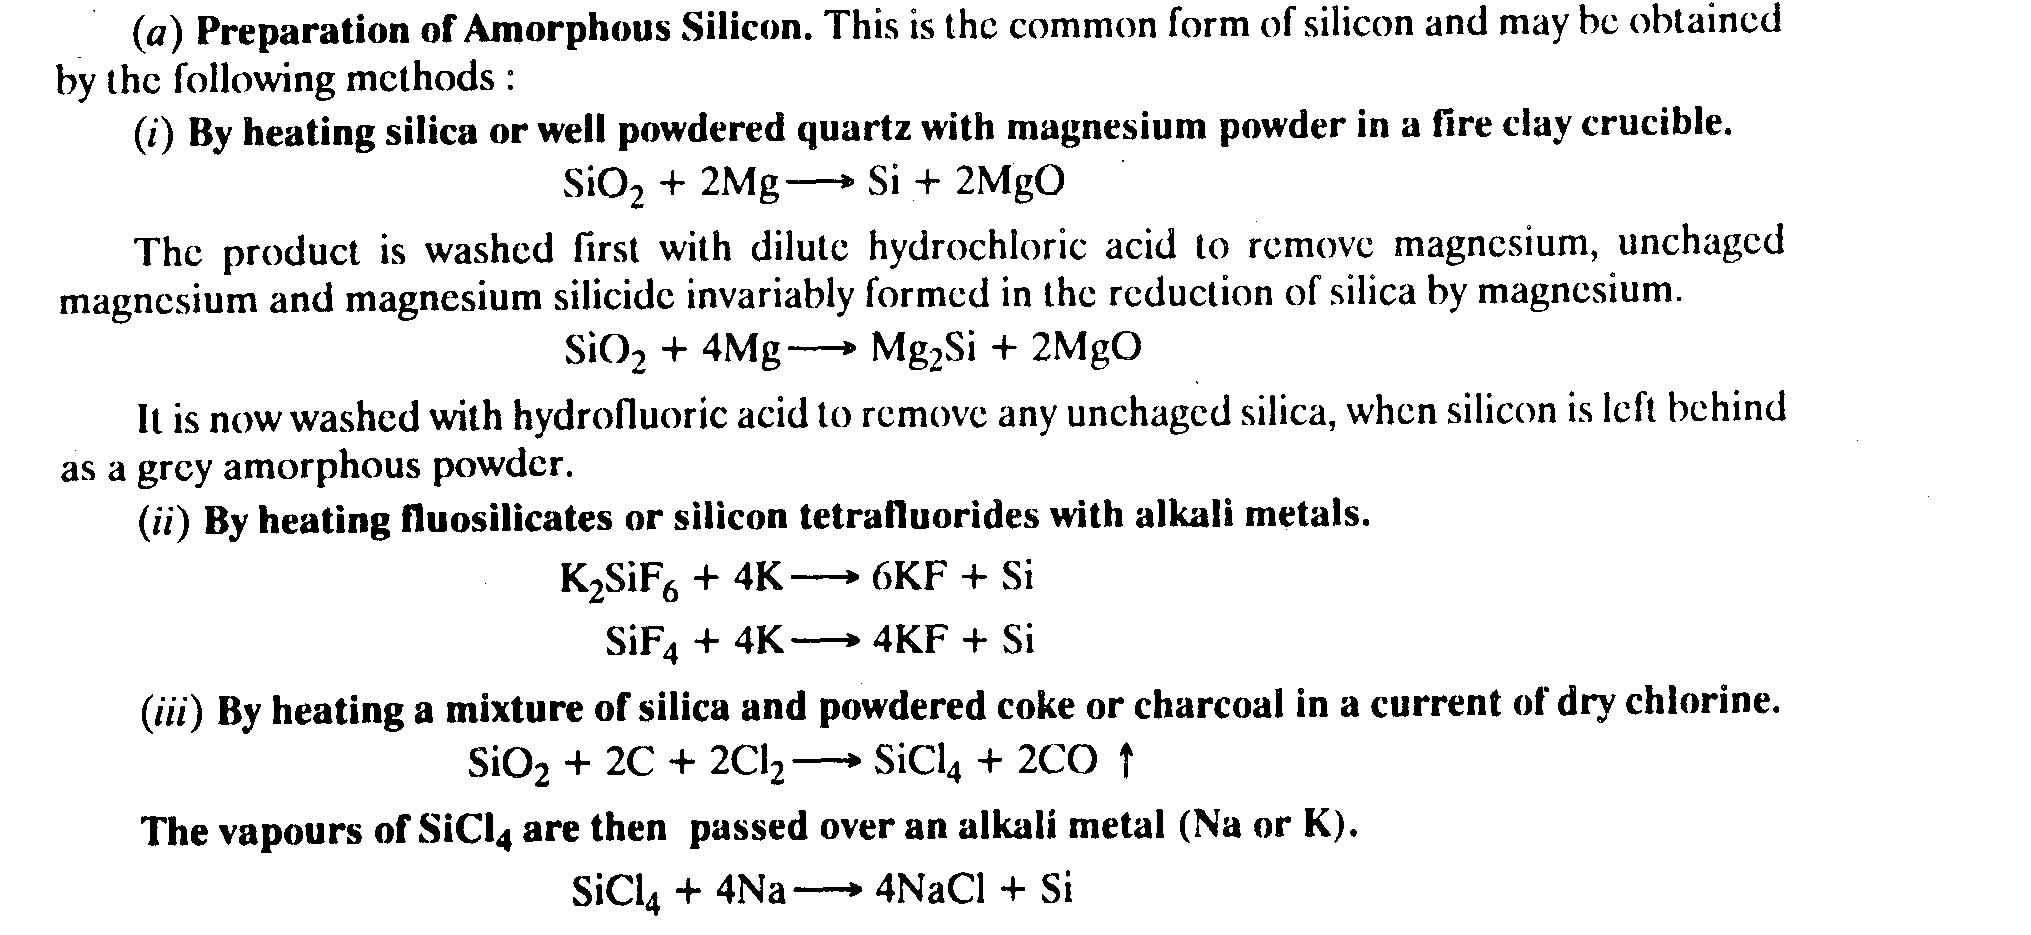
\includegraphics[width=0.22\textwidth]{sampleDocument.png} &
 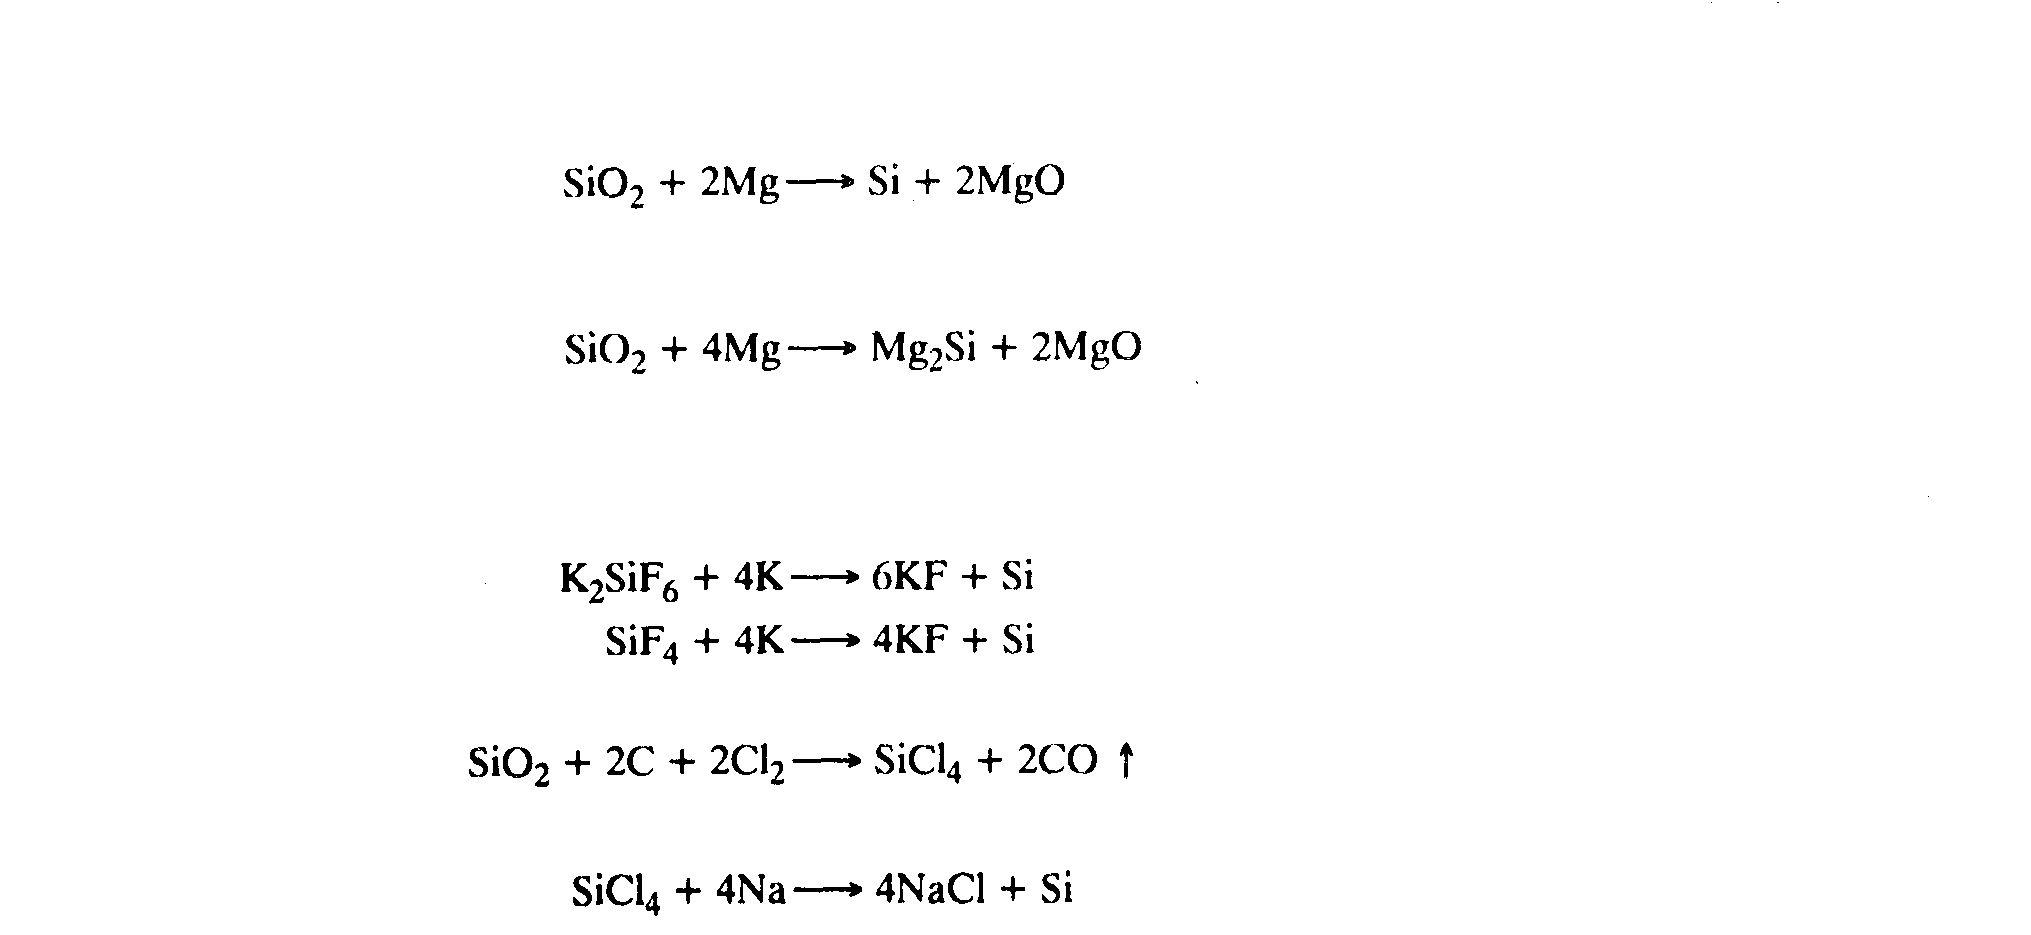
\includegraphics[width=0.22\textwidth]{DCE.png} \\
(a)  & (b) \\ 
%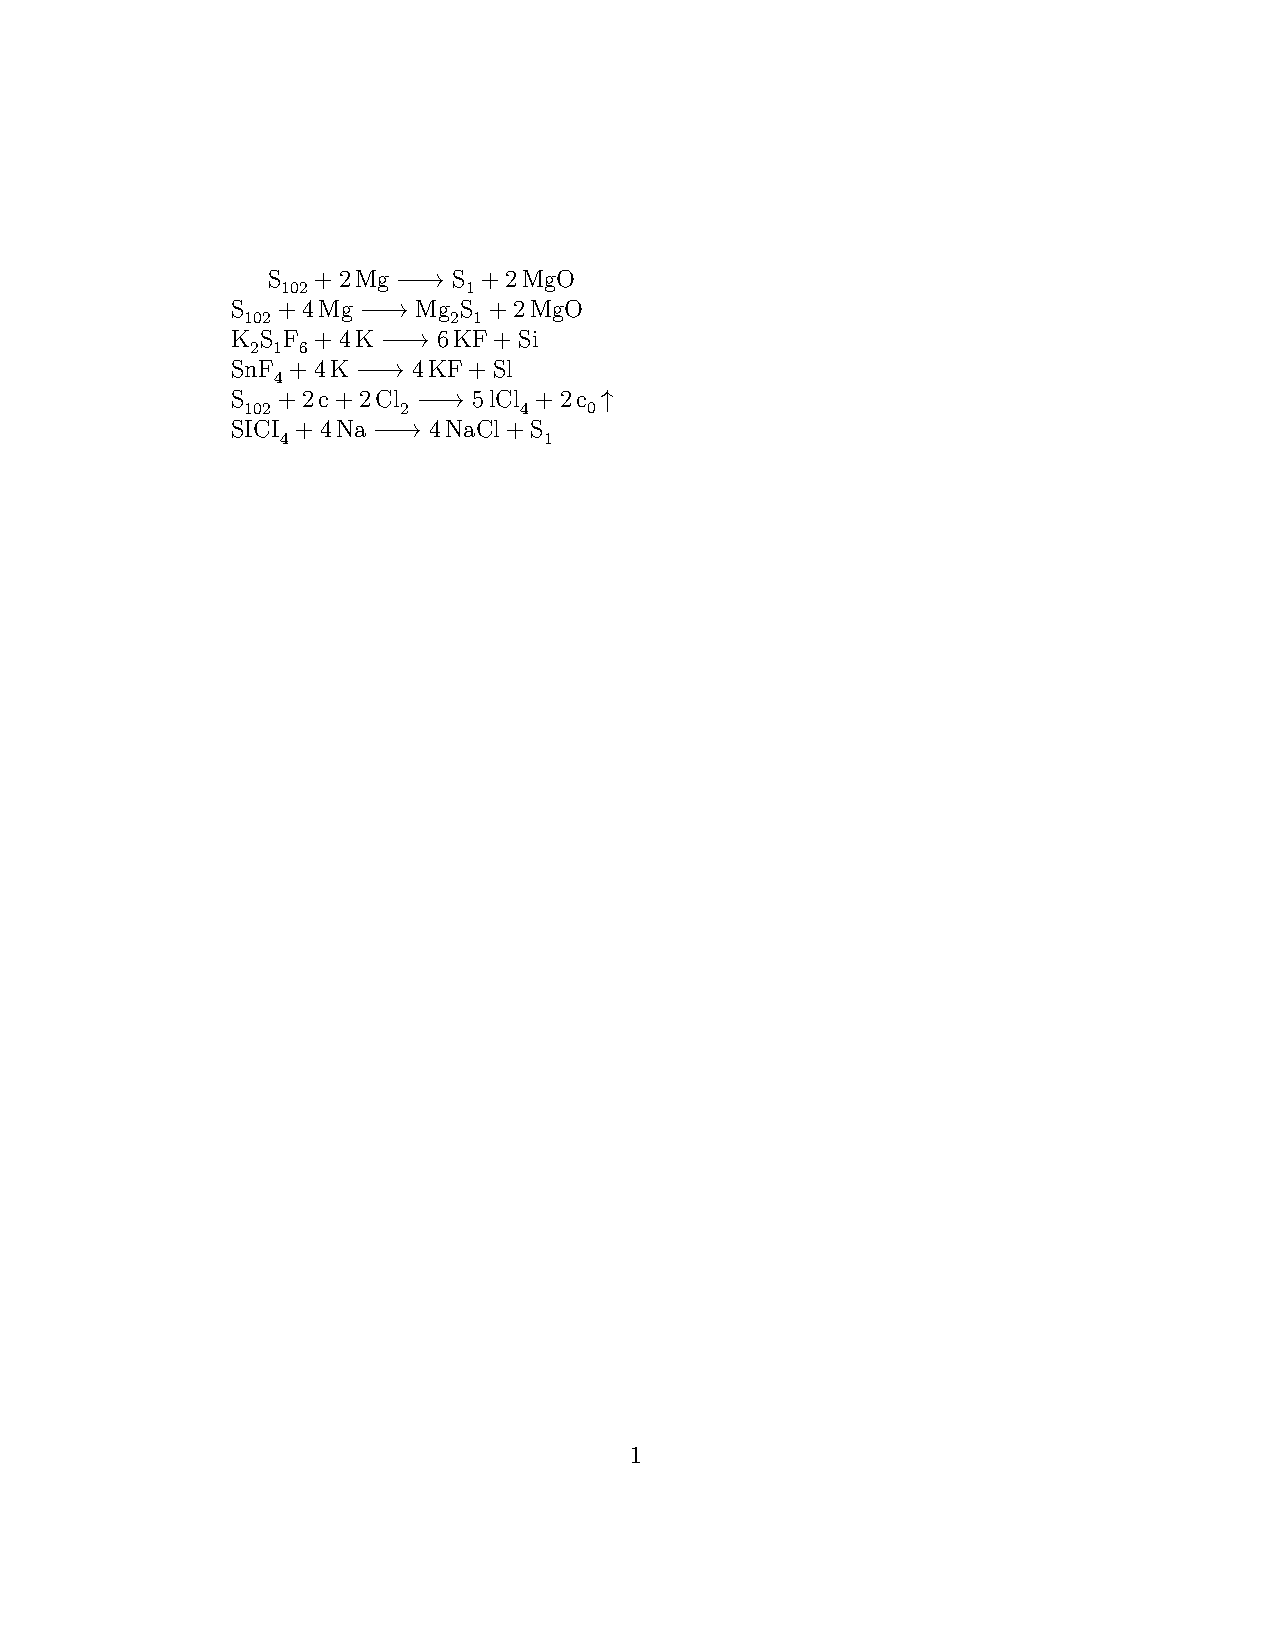
\includepdf[(pages={1})]{ directOCR.pdf } \\
\hline
 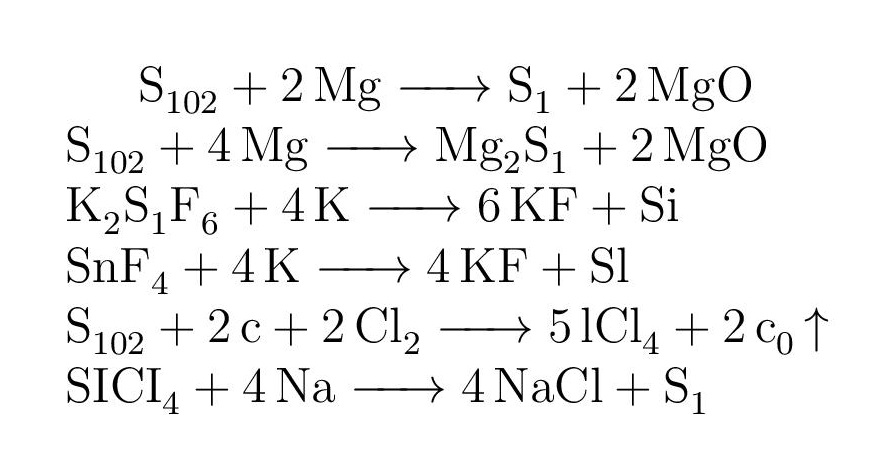
\includegraphics[width=0.2\textwidth]{directOCR.jpg} &
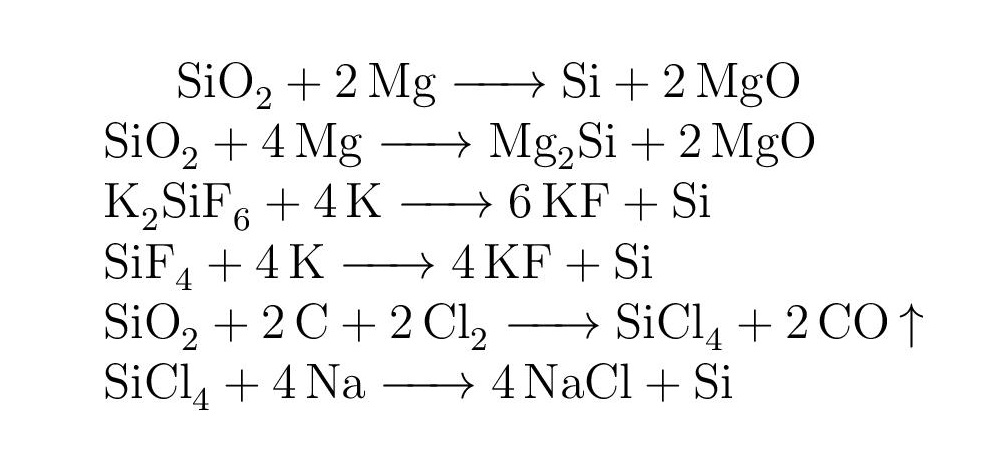
\includegraphics[width=0.2\textwidth]{correctedFinalEq.jpg}\\
 
 (c)  & (d)  \\
 \hline
\end{tabular}
\caption{Experimental result; (a) Input image; (b) Segmented Chemical equation;
(c) OCR output in PDF format; (d) Output of the proposed method.}
\label{eg} 
\end{figure}
\section{Experimental Result}
We have implemented our algorithm in MATLAB 8.3.0.532
(R2014a) in a PC (Intel(R) Core(TM) i5-3337U CPU @ 1.80GHz
running Windows 8). The proposed method has been tested on
a dataset consisting 234 document pages. Out of 234 pages 50
pages are taken from ICDAR 2013 Math-zone segmentation
datasets and other document pages are scanned from different Mathematics and
Chemistry books. 
The summary of the experimental results
is shown in Table~\ref{table:result}. Out of 3406 chemical compounds in the test dataset, 114 were partially corrected and 52 could not be corrected at all. The overall accuracy of autocorrection is 95.12\%. These results are quite encouraging. See the sample image (Fig.~\ref{eg}(a)). Corresponding segmented displayed chemical equations are shown in Fig.~\ref{eg}(b). Fig.~\ref{eg}(c) shows the direct OCR output where `i' has been wrongly identified as `l', `I' and `1' (for $Si$ in all the lines of  Fig.~\ref{eg}(c)). Similarly `O' results in `0' (line 1,2,3). `S' sometimes is detected as `5' (line 5). Our auto correction algorithm remedies these issues. Fig.~\ref{eg}(d) demonstrates the effect of our auto correction algorithm. This algorithm is targeted towards chemical equation with linear representation.
It fails when the chemical equation contains some text such as $and$, $or$ etc between two displayed equation in the same line. Also, when the chemical compound is written in formats such as $(Na_2SiO_3)_n$, only $Na_2SiO_3$ is detected based on $ChemList$. Some equations have conditions (pressure, temperature) written over the arrows. We have not ventured in that yet. But the error case that has been mentioned in Algorithm~\ref{alg:alg3} has very less probability of occurrence. Hence it is ignored.



%\begin{table}[h]
%\captionof{table}{Summary of Experimental Results}
%\centering
%\begin{tabular}{|c|c|l|c|}
%\cline{1-2} \cline{4-4}
%{\color[HTML]{000000} \# Total Images}                     & 234     &  &                                                                                          \\ \cline{1-2}
%{\color[HTML]{000000} \# Total DEs}                        & 1390    &  & \multirow{-2}{*}{\begin{tabular}[c]{@{}c@{}}Operator Recognition\\ 98.83\%\end{tabular}} \\ \cline{1-2} \cline{4-4} 
%{\color[HTML]{000000} DE segmentation accuracy}            & 98.63\% &  &                                                                                          \\ \cline{1-2}
%{\color[HTML]{000000} Chemical DE Classification Accuracy} & 98.83\% &  & \multirow{-2}{*}{\begin{tabular}[c]{@{}c@{}}Auto Correction\\ 95.12\%\end{tabular}}      \\ \cline{1-2} \cline{4-4} 
%\end{tabular}
%\label{table:result}
%\end{table}


\begin{table}
\captionof{table}{Summary of Experimental Results}
\begin{center}
 \begin{tabular}{| c | c |}
 \hline
 \#Total DEs & 1390\\
 \hline
Operator recognition & 98.83\% \\
\hline
 DE segmentation accuracy & 98.63\% \\
 \hline
Chemical DE Classification Accuracy & 98.83\%\\
\hline 
Auto correction accuracy & 95.12\% \\
\hline

 \end{tabular}
 \end{center}
 \label{table:result}
 \end{table}

%%%%%%%%%%%%%%%%%%%%%%%%%%%%%%%%%%%%%%%%

\section{Conclusion}
We have presented an automated chemical equation segmentation and chemical context based auto correction system that is able to provide the exact searchable format of linear chemical equations in any document image. The experimental results demonstrate the efficiency of our proposed method. This work leads to several research avenues. Chemical context horizon can be widened. Auto correction on non-linear or bond structure representations of chemical equations could be ventured in.










\begin{thebibliography}{1}

%\bibitem{IEEEhowto:kopka}
%H.~Kopka and P.~W. Daly, \emph{A Guide to \LaTeX}, 3rd~ed.\hskip 1em plus
  %0.5em minus 0.4em\relax Harlow, England: Addison-Wesley, 1999.

\bibitem{spc_07} S.~P.~Chowdhury, S.~Mandal, A.~K.~Das, and
B.~Chanda, \emph{Segmentation of Text and Graphics from Document
Images}, In Proc. of ICDAR, pp. 619–623,2007.

\bibitem{sekhar_06} S.~Mandal, S.~P.~Chowdhury, A.~K.~Das, and
B.~Chanda, \emph{A simple and effective table detection system
from Document Images}, IJDAR, Vol. 8(2), 172–182, 2006.

\bibitem{blostein_97} D.~Blostein and A.~Grabavec,
\emph{Recognition of Mathematical Notation}, Handbook of
Character Recognition and document Image Analysis, 577--582,
1997.
 
\bibitem{chan_00} K-F.~Chan and D-Y.~Yeung, \emph{Mathematical
Expression Recognition: A Survey}, IJDAR, Vol. 3, no: 1, 3–15,
2000.

\bibitem{Garain_07} U.~Garain and B.~B.~Chaudhuri \emph{An OCR
of Printed mathematical Expressions, Digital Document
Processing}, Ed: B.~B.~Chaudhuri, Advances in pattern
Recognition, 235–259 , 2007.

\bibitem{uchid_10}
A.~Fujiyoshi, M.~Suzuki, S.~Uchid,
 \emph{Grammatical Verification for Mathematical Formula Recognition Based on Context-Free Tree Grammar},
 Mathematics in Computer Science, 279--298, 2010.
 
 
 \bibitem{algorri_07}
 M.~E.~Algorri, M.~Zimmermann, C.~M.~Friedrich, S.~Akle, and M.~Hofmann-Apitius,
\emph{Reconstruction of chemical molecules from images},
In Proc. 29th Annual International IEEE Conference on Engineering in
Medicine and Biology Society, 4609--4612, 2007.

\bibitem{algorri_07a}
M.~E.~Algorri, M.~Zimmermann, and M.~Hofmann-Apitius,
\emph{Automatic recognition of chemical images},
In pro. Eighth Mexican International Conference on Current Trends in Computer Science, 41--46, 2007.
\bibitem{park_09}
J.~Park, G.~R.~Rosania, K.~A.~Shedden, M.~Nguyen, N.~Lyu, and K.~Saitou,
\emph{Automated extraction of chemical structure information from digital raster images}, Chemistry Central journal, vol. 3(1), 2009.

\end{thebibliography}




% that's all folks
\end{document}


